\section{Large-Scale Trial on Whole Sentinel-2 Products}
\label{app:large_scale_trial}
The study above compresses one band of one tile per region. This appendix
runs the operational chain end to end on ten whole Sentinel-2 L2A products,
every band and every group of the product, and measures what a reader of
the archive would see: the size of the stored product and the error on the
native pixels.

\paragraph{Products and chain}
The ten products are EOPF Zarr products of the 2026 sample service, chosen
for varied landscapes from urban to open sea, high mountain, arid
greenhouses and boreal lakes (Table~\ref{tab:operational_sizes}), with
cloud cover below $4\%$ except the volcanic and glacier tile ($78\%$).
Each product is converted to HEALPix with the legacy-converters preset:
the reflectance at \SI{10}{m}, \SI{20}{m} and \SI{60}{m} goes to levels 20,
19 and 17 by the PSF-aware \term{transfer}~\cite{delouis2026resample}
(9 nearest pixels per cell, weight threshold $0.1$, damping
$\lambda=0.1$, at most 100 conjugate-gradient iterations), one level-11
cell per chunk ($4^9$, $4^8$ and $4^6$ cells), and is stored under the
\texttt{hcc-sentinel2-pyramid} codec described below. Masks, scene
classification, atmosphere, probabilities and footprints are transferred
by nearest neighbour and stored losslessly; geometry, meteorology and
metadata are carried over.

\paragraph{The Sentinel-2 codecs}
Both codecs work on the digital numbers (DN) of the product,
$\mathrm{DN}=\mathrm{round}(Q\rho-O)$, with $Q=10^4$ and $O=-1000$ read
from the product's scale factor and offset, so that 1~DN is $10^{-4}$ in
reflectance; DN 0 is the no-data number and valid values are clipped to
$[1, 65535]$. A chunk, one nested level-11 cell holding $4^\delta$ cells,
is de-interleaved into its $2^\delta\times2^\delta$ raster in face
indices, the image a JPEG~XL coder expects.
\begin{itemize}
\item \texttt{hcc-sentinel2} stores that raster of DN under lossless
  JPEG~XL (effort 7). Its only error is the rounding to the DN lattice,
  of RMS $1/(Q\sqrt{12})$. The trial uses it for the aerosol optical
  thickness, the water vapour, the scene classification and the cloud and
  snow probabilities, with the lattice shifted by one where 0 is a valid
  value.
\item \texttt{hcc-sentinel2-pyramid} stores the reflectance in two layers.
  The \emph{base} is the parent level: the mean of the valid children of
  each parent, rounded to the DN lattice and coded with lossless JPEG~XL,
  so the parent level is exact up to that rounding. The children are
  predicted from the decoded base, one least-squares filter per child
  position (four in all) over the $5\times5$ neighbourhood of parents
  plus a constant, fitted on the chunk's fully valid parents; the 104
  coefficients are stored with the chunk. The \emph{detail}, children
  minus prediction in DN, is quantised with a uniform step
  $s=\max(s_{\min}, r\,\sigma)$, where $\sigma$ is the standard deviation
  of the chunk's detail, $r=0.57$ and $s_{\min}=1$~DN, and coded with
  lossless JPEG~XL. The error of every cell is at most $s/2$. The validity
  of the children of partly valid parents is kept as a bit mask, so
  no-data cells round-trip as no-data.
\end{itemize}
The step follows the detail of each chunk, so a rough chunk gets a coarse
step and a smooth one a fine step, as an error budget proportional to the
local \term{transfer} error asks. On B04 of T31UDQ, $r=0.36$ puts the
added error at the \term{transfer} error, for about $1.5$ times the
lossless JPEG~2000 tile; the default $r=0.57$ aims at $1.5$ times the
\term{transfer} error for about $1.3$ times that size. The other groups
keep the converter's default lossless coding. The final conversion pass, which converted the reflectance
again (see below), took $5.1$ to $5.3$~h of wall time per product on one
JupyterHub server shared by products converted concurrently, quality
measurement excluded.

\paragraph{Size}
Table~\ref{tab:operational_sizes} compares the HEALPix product with the
EOPF product as distributed and with the reflectance of the UTM tile under
lossless JPEG~2000, the SAFE baseline. Over the ten products, the
HEALPix reflectance is $1.50$ times the lossless JPEG~2000 reflectance
($1.48$ in median, $1.36$ to $1.90$ by tile) and $1.16$ times the EOPF
reflectance; the other groups grow from 915 to 1\,043~MB;
the whole product grows from 10.7 to 12.4~GB, by $16\%$.
The codec's default was set for about $1.3$ times the lossless
JPEG~2000 size on B04 of T31UDQ; the same tile measures $1.31$ at
\SI{10}{m} here. The ratio is highest where the UTM tile is cheapest:
the arid tile ($1.90$) and the coastal tile with open sea ($1.70$), whose
smooth or partly empty UTM rasters compress well while the HEALPix
\term{carrier} holds the detail the deconvolving \term{transfer} restores.

\begin{table*}[t]
\centering
\caption{Whole Sentinel-2 L2A products, EOPF Zarr as distributed against the HEALPix Zarr of the operational chain (legacy-converters preset, reflectance under \texttt{hcc-sentinel2-pyramid} with $r=0.57$). Sizes in MB. JP2: the UTM reflectance under lossless JPEG~2000 per source chunk, the SAFE reference. ``Other'': masks, classification, atmosphere, probabilities, footprints, geometry, meteorology, metadata.}
\label{tab:operational_sizes}
\small
\begin{tabular}{llrrrrrrrr}
\toprule
 & & \multicolumn{4}{c}{Reflectance (all bands, 10/20/60~m)} & \multicolumn{2}{c}{Other groups} & \multicolumn{2}{c}{Whole product} \\
\cmidrule(lr){3-6}\cmidrule(lr){7-8}\cmidrule(lr){9-10}
Landscape & Tile & EOPF & JP2 & HEALPix & $\times$JP2 & EOPF & HEALPix & EOPF & HEALPix \\
\midrule
Urban, cropland & T31UDQ & 1\,134 & 861 & 1\,169 & 1.36 & 126 & 141 & 1\,260 & 1\,310 \\
High mountain, snow & T32TLR & 1\,148 & 877 & 1\,218 & 1.39 & 147 & 160 & 1\,295 & 1\,378 \\
Irrigated cropland & T30STG & 1\,126 & 857 & 1\,250 & 1.46 & 130 & 173 & 1\,256 & 1\,424 \\
Pine forest & T30TXP & 981 & 788 & 1\,126 & 1.43 & 108 & 105 & 1\,089 & 1\,232 \\
Arid, greenhouses & T30SWF & 738 & 573 & 1\,089 & 1.90 & 33 & 43 & 771 & 1\,132 \\
Coast, open sea & T30UUU & 785 & 620 & 1\,052 & 1.70 & 31 & 30 & 815 & 1\,082 \\
Port, delta & T31UET & 840 & 667 & 1\,019 & 1.53 & 48 & 50 & 888 & 1\,069 \\
Volcanic, glacier & T27VWL & 917 & 725 & 1\,118 & 1.54 & 61 & 70 & 978 & 1\,188 \\
Wetlands, lagoons & T31TFJ & 1\,093 & 844 & 1\,154 & 1.37 & 120 & 126 & 1\,213 & 1\,280 \\
Boreal forest, lakes & T35VNK & 1\,001 & 782 & 1\,167 & 1.49 & 111 & 145 & 1\,112 & 1\,313 \\
\midrule
All 10 & & 9\,763 & 7\,595 & 11\,363 & 1.50 & 915 & 1\,043 & 10\,678 & 12\,406 \\
\multicolumn{5}{l}{Median (min--max) of $\times$JP2 over tiles} & 1.48 (1.36--1.90) & & & & \\
\bottomrule
\end{tabular}
\end{table*}


\paragraph{Quality}
The error is measured on the native UTM pixels of 12 random interior
level-11 chunks per tile and resolution, with the observation operator of the
\term{transfer} (Table~\ref{tab:operational_quality}). The \term{transfer}
alone leaves $5$ to $6$~DN RMS at \SI{10}{m}, under $1\%$ of the scene's
standard deviation; the codec adds $1.55$ times that error in median at
\SI{10}{m} and \SI{20}{m}, the ratio its default was designed for. Per
tile and band, the ratio stays within $1.39$ to $1.63$ at \SI{10}{m}
and within $1.42$ to $1.81$ at \SI{20}{m} on all ten tiles, except B01, a \SI{60}{m} band resampled to \SI{20}{m} by the
product, whose \term{transfer} error is below 1~DN (up to $2.57$). At
\SI{60}{m} the ratio falls to $0.65$: at level 17 the \term{transfer}
error dominates, about four times its value at \SI{20}{m} for the bands
present at both resolutions, while the codec's step follows the residual
and not that error.

\begin{table}[t]
\centering
\caption{Error on the native UTM pixels of the ten products, in digital numbers (1~DN $=10^{-4}$ reflectance), on 12 random interior level-11 chunks per tile and resolution: standard deviation of the native pixels, error of the PSF transfer alone, error added by \texttt{hcc-sentinel2-pyramid} (stored against uncompressed transfer, both read back with the transfer's operator) and total. RMS over the tiles; the last column is the median (min--max) over the tiles of added/transfer.}
\label{tab:operational_quality}
\small
\setlength{\tabcolsep}{3.5pt}
\begin{tabular}{llrrrrl}
\toprule
Res. & Band & $\sigma$ & Transfer & Added & Total & Added/transfer \\
\midrule
10m & B02 & 645 & 5.3 & 7.7 & 9.4 & 1.57 (1.40--1.61) \\
10m & B03 & 663 & 5.2 & 7.7 & 9.3 & 1.56 (1.40--1.63) \\
10m & B04 & 735 & 5.1 & 7.4 & 9.0 & 1.55 (1.39--1.62) \\
10m & B08 & 822 & 6.2 & 9.4 & 11.2 & 1.52 (1.41--1.63) \\
\midrule
20m & B01 & 480 & 0.9 & 1.5 & 1.8 & 1.69 (1.57--2.57) \\
20m & B02 & 617 & 8.6 & 12.7 & 15.4 & 1.55 (1.45--1.62) \\
20m & B03 & 636 & 8.6 & 12.8 & 15.4 & 1.58 (1.46--1.63) \\
20m & B04 & 709 & 8.7 & 13.1 & 15.7 & 1.56 (1.46--1.62) \\
20m & B05 & 699 & 6.9 & 10.4 & 12.5 & 1.57 (1.46--1.63) \\
20m & B06 & 716 & 7.3 & 11.1 & 13.3 & 1.56 (1.42--1.63) \\
20m & B07 & 759 & 7.5 & 11.6 & 13.8 & 1.56 (1.42--1.62) \\
20m & B11 & 668 & 4.2 & 6.4 & 7.6 & 1.51 (1.42--1.65) \\
20m & B12 & 582 & 3.9 & 6.1 & 7.2 & 1.53 (1.44--1.64) \\
20m & B8A & 773 & 7.2 & 11.0 & 13.2 & 1.55 (1.42--1.63) \\
\midrule
60m & B01 & 420 & 10.2 & 7.6 & 12.8 & 0.78 (0.70--0.87) \\
60m & B02 & 475 & 29.1 & 17.3 & 33.8 & 0.64 (0.55--0.69) \\
60m & B03 & 497 & 30.1 & 18.1 & 35.3 & 0.65 (0.55--0.69) \\
60m & B04 & 580 & 33.4 & 20.8 & 39.6 & 0.65 (0.55--0.69) \\
60m & B05 & 575 & 33.3 & 20.7 & 39.3 & 0.66 (0.55--0.70) \\
60m & B06 & 600 & 36.3 & 22.7 & 42.9 & 0.64 (0.57--0.70) \\
60m & B07 & 659 & 39.3 & 25.0 & 46.6 & 0.64 (0.57--0.69) \\
60m & B09 & 665 & 28.3 & 19.7 & 34.5 & 0.70 (0.64--0.75) \\
60m & B11 & 612 & 32.7 & 21.7 & 39.3 & 0.66 (0.55--0.71) \\
60m & B12 & 540 & 29.6 & 19.7 & 35.7 & 0.65 (0.56--0.72) \\
60m & B8A & 685 & 39.9 & 25.5 & 47.4 & 0.64 (0.58--0.69) \\
\bottomrule
\end{tabular}
\end{table}


\paragraph{Spectral check}
The table scores the error as a number; its spectrum says whether the
compressed product carries structure the source does not.
Figure~\ref{fig:s2_ten_tiles_overview} shows each stored product as a
reader sees it, the level-17 reflectance drawn on the tile's own
\SI{60}{m} grid, with ten random $256\times256$ patches of
\SI{10}{m} pixels per tile, drawn among those with at most $0.1\%$ of
no-data pixels. Figure~\ref{fig:s2_ten_tiles_spectra} gives three radial
power spectra for each patch and \SI{10}{m} band: the UTM source; the
residual of the source minus the stored HEALPix field read back onto the
same pixels with the \term{transfer}'s own observation model, which holds
the \term{transfer} and compression errors together; and the stored
HEALPix cells themselves, on the plane tangent to the patch centre,
where the nested cells form a regular grid in face indices, so the
Fourier transform is taken on that grid without interpolation. The HEALPix
spectrum follows the source up to the UTM Nyquist frequency, and the
residual is flat, white noise with no peak at the chunk size or at any
other scale; it lies up to six orders of magnitude below the signal at
kilometre scales and meets it only near the UTM Nyquist frequency on the
smoothest patches. In the median over the patches of a tile, the RMS
of the residual, \term{transfer} and compression together, is $0.03$ to
$1.5\times10^{-3}$ in reflectance, $19$ to $141$ times below the patch's
standard deviation by tile and band.

\begin{figure*}[t]
\centering
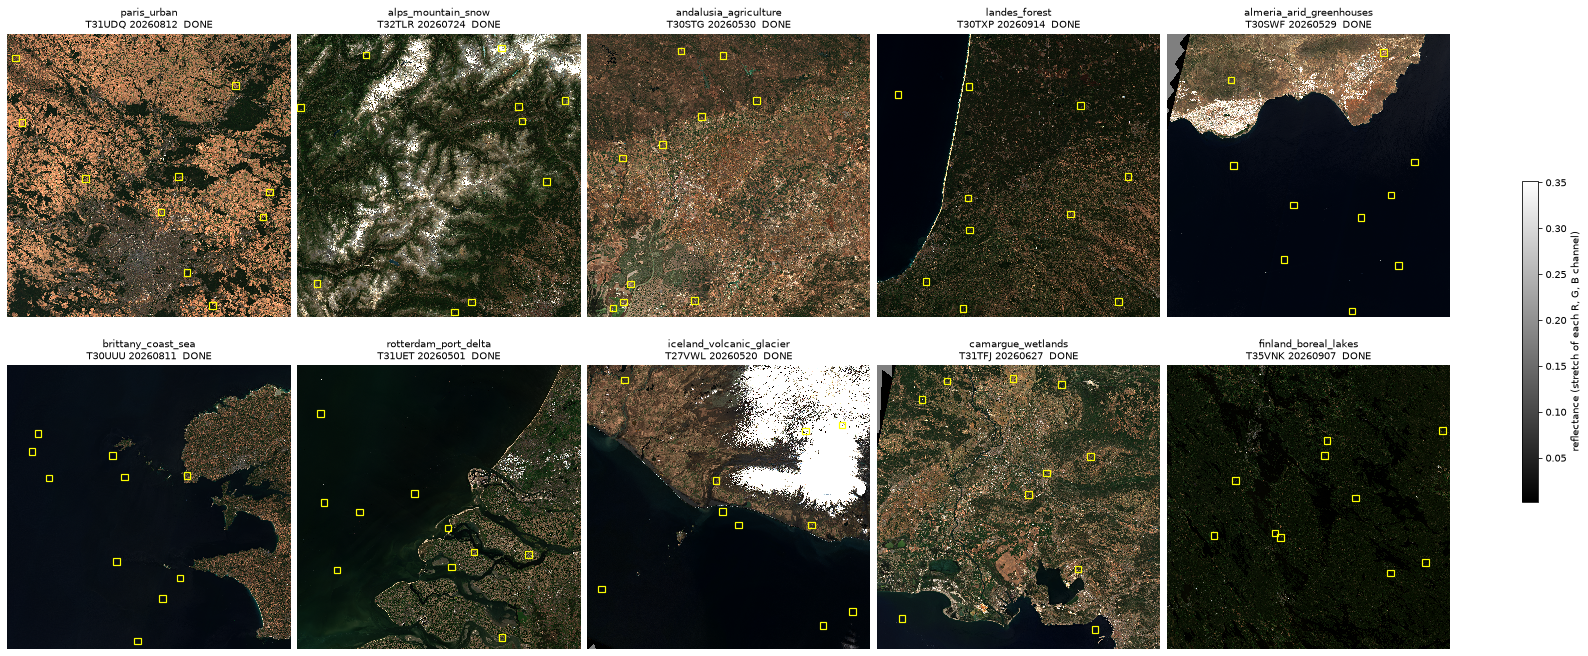
\includegraphics[width=\textwidth]{figures/fig_s2_ten_tiles_overview}
\caption{The ten HEALPix products of the large-scale trial as stored:
B04/B03/B02 composite of the level-17 reflectance on each tile's
\SI{60}{m} UTM grid, one contrast stretch for all tiles (colour bar).
Yellow squares: the $256\times256$ patches of
Fig.~\ref{fig:s2_ten_tiles_spectra}.}
\label{fig:s2_ten_tiles_overview}
\end{figure*}

\begin{figure*}[t]
\centering
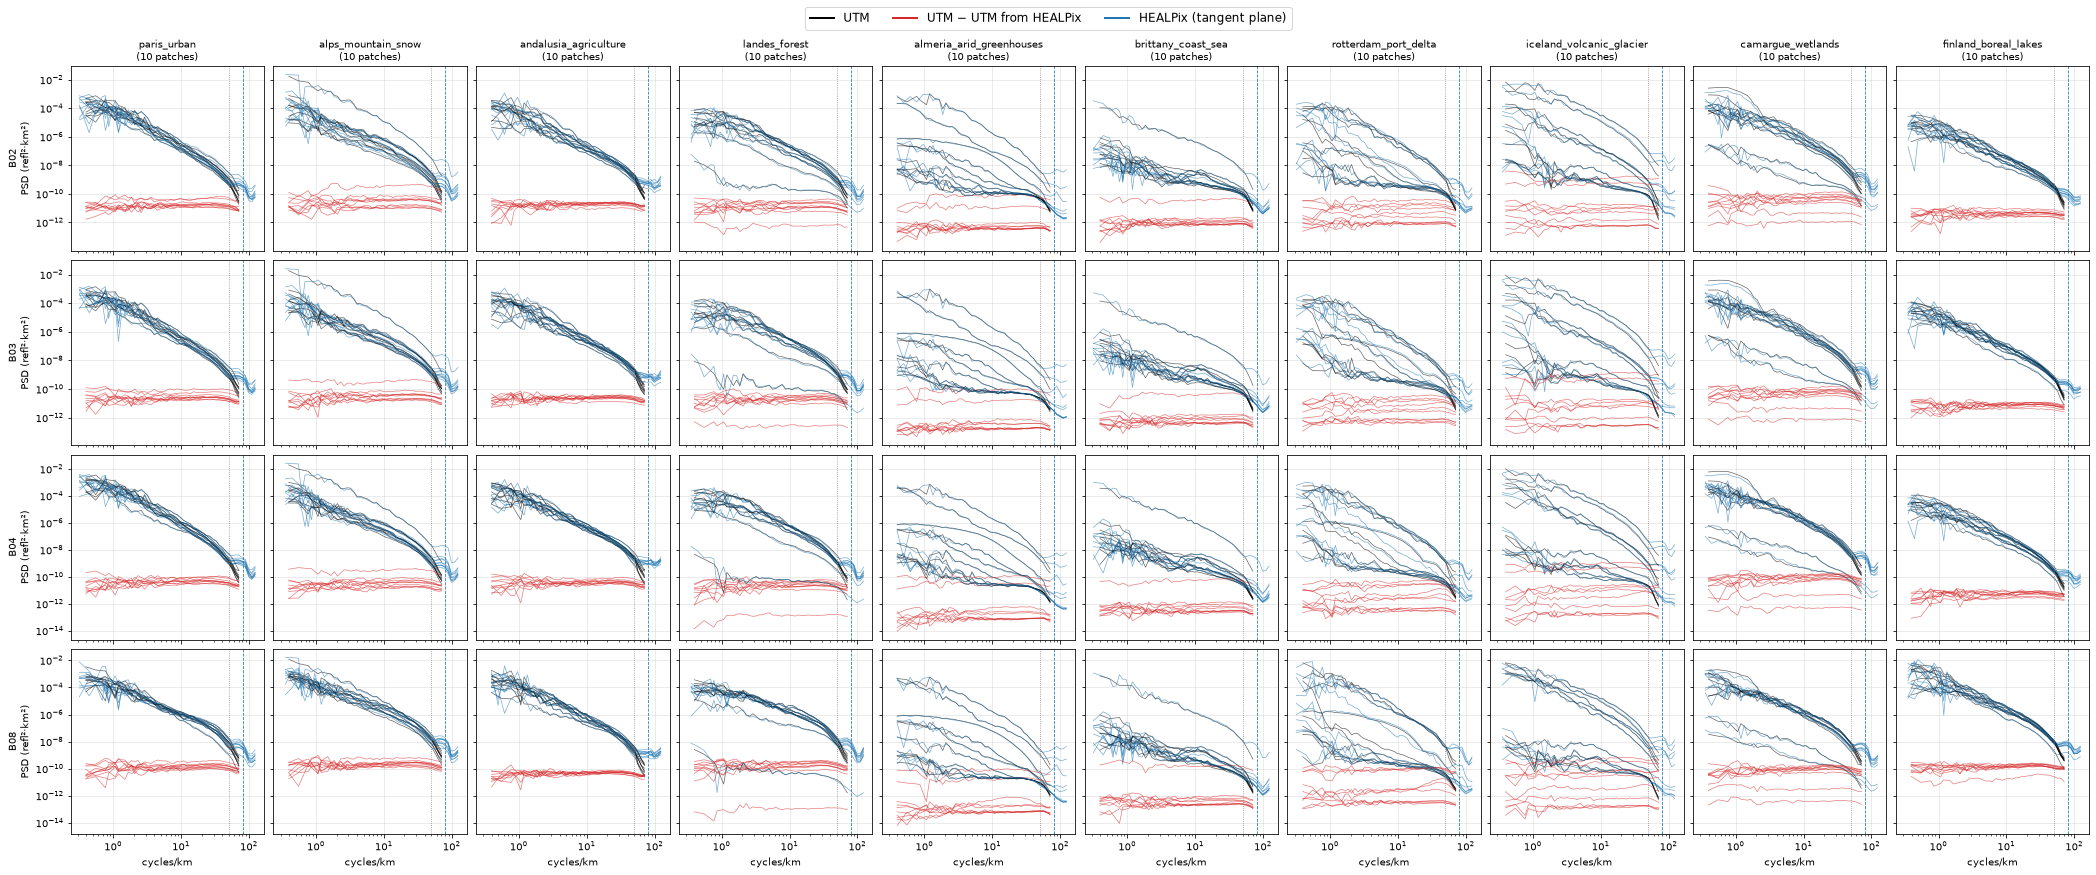
\includegraphics[width=\textwidth]{figures/fig_s2_ten_tiles_spectra}
\caption{Radial power spectra of the \SI{10}{m} bands (rows) of the ten
products (columns), one line per patch of
Fig.~\ref{fig:s2_ten_tiles_overview}, in reflectance$^2\,$km$^2$. Black:
UTM source. Red: source minus the compressed HEALPix field read back onto
the UTM pixels with the PSF model of the \term{transfer}. Blue:
compressed HEALPix cells on the tangent plane. Dotted: UTM Nyquist
frequency (50~cycles/km); dashed: Nyquist frequency of the
level-20 index grid.}
\label{fig:s2_ten_tiles_spectra}
\end{figure*}

\paragraph{No-data pixels inside a tile}
The measurement must leave out the pixels a product flags as no-data, as
the conversion does. Over the boreal lakes of T35VNK, some B02 pixels
inside the tile carry the no-data number 0, which the reflectance
encoding also gives to values below $-0.1$: 227 of the sampled pixels,
196 of them in one chunk, and a few in B03, B04 and B08; two other
tiles have a few (16 on B08 of T30STG, 4 on B02 of T27VWL). The conversion reads them as missing and the
\term{transfer} leaves them out. A first version of the measurement
scored them as reflectances of $-0.1$, in its uncompressed \term{transfer}
and in the native pixels alike, and reported an added error of $10.2$
times the \term{transfer} error on that band (and $1.94$ on B08 of
T30STG). The stored product was not at fault: on the affected chunk, it
departs from a \term{transfer} that leaves the no-data pixels out by the
codec's own error ($3$~DN RMS on B02).
Table~\ref{tab:operational_quality} is measured that way, with each
band's no-data pixels excluded.

\paragraph{What the trial exposed}
Running whole products surfaced defects that single-band tiles had not.
In the first pass, a single invalid pixel turned a whole band invalid in
the \term{transfer} of healpix-resample v2026.6.0, and the batched
conversion spread it to the other bands of the chunk, leaving four tiles
with missing chunks; the reflectance of all ten products was converted
again with the fixed release ($\ge$ v2026.7.0), and the tables above come
from that conversion. The other defects found along the way, in the
\term{transfer}, the converter and the processing image, were reported
to the packages concerned, with fixes.

\paragraph{Scope of this appendix}
This trial lies outside the deposited chain. It ran the operational
packages, the EOPF reader, the converter, \texttt{healpix-resample} and
the two codecs, on products held on an object store, and the HEALPix
products it wrote stay on that store. The notebook that measured the two
tables and drew the two figures is in the repository
(\texttt{test/validation\_s2\_ten\_tiles.ipynb}); its inputs are not in
the data deposit, \texttt{reproduce.sh} does not run it, and the checker
of Section~\ref{sec:reproducibility} does not assert the figures quoted
here. They are reported as the outcome of one production run.
